\chapter{O Projeto}
\label{chapter:projeto}

Os dois últimos capítulos descreveram o conceito de Internet das Coisas e as especificações que o projeto deve contemplar, visando sempre ajudar na construção de sistemas IoT que melhor se encaixem na aplicação. Neste capítulo serão descritos as implementações do projeto, apresentado os motivos das escolhas de tecnologias e protocolos especificados. E terminando sobre persistência de dados em aplicações IoT e por quê a escolha de implementação bancos de dados é importante para a aplicação.


\section{Camada de Abstração}
\label{section:camada_abstracao}

Devido a interação entre dispositivos de aquisição de dados e aplicação e armazenamento de dados, foi necessário uma implementação de um protocolo de comunicação único entre os dispositivos e implementação em cada um destes em suas diferentes linguagens de programação.

O protocolo consiste em uma abstração de um canal de envio de dados chamado Data Stream mostrado em \ref{fig:3.1.0/data_stream}, no qual passam dados após realizar um processamento dos dados em uma determinada velocidade podendo conter um limite de pacote de dados. Nas pontas desse canal estão os Publishers e Subscribers, que serão descritos adiante. Este conceito é uma forma de abstrair, unificar e simplificar a forma de transporte de dados, de uma modo que a interface possa ter o controle sobre os aspectos de transmissão. Cada protocolo na camada de aplicação, implementa este conceito de uma certa forma, porém o desenvolvedor não precisará se preocupar com estes detalhes.


\section{Publishers e Subscribers}
\label{section:publishers_subscribers}

Para enviar e receber dados de uma forma a atender os requisitos da seção \ref{section:interface}, foi utilizado um padrão de comunicação recorrente em aplicações contemporâneas, o padrão Publish/Subscriber \cite{amazon:pub-sub}.

O padrão Publish/Subscribe permite que as mensagens sejam transmitidas assíncronas e para vários dispositivos simultaneamente. Para transmitir uma mensagem, um client pode simplesmente enviar uma mensagem para o tópico que os envia imediatamente para todos os subscribers. Todos os componentes que se inscreverem no tópico receberão todas as mensagens transmitidas, a menos que uma política de filtragem de mensagens seja definida pelo assinante.

\begin{figure}[h!]
\centering
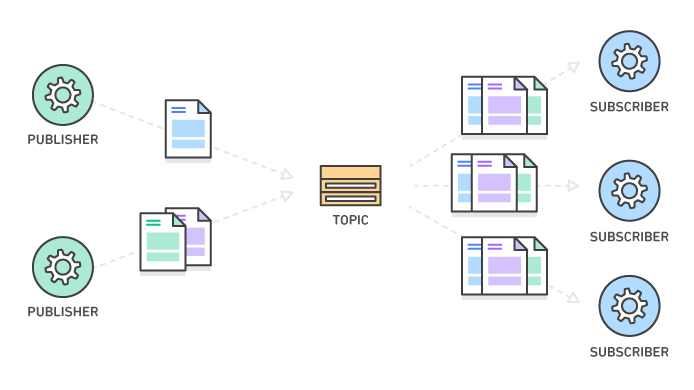
\includegraphics[width=12cm]{./02_Capitulos/02_Cap3/figures/aws_pub_sub}
\caption{O padrão Publish/Subscribe. Retirado de \cite{amazon:pub-sub}}
\label{fig:3.2.0/aws_pub_sub}
\end{figure}

Qualquer mensagem publicada em um tópico é imediatamente recebida por todos os subscribers do tópico. As mensagens de podem ser usadas para arquiteturas orientadas a eventos ou para desacoplar aplicativos, aumentando  o desempenho, a confiabilidade e a escalabilidade. Com isso, foram criados duas funções possíveis para cada dispositivo dentro deste padrão, os Publishers e os Subscribers, sua comunicação é descrita em \ref{fig:3.2.0/pub_sub}.


Publishers são dispositivos que criam Data Stream  e enviam dados por estes, regulam o processamento dos dados estipulam limites de tamanho de cada pacote de dado e determinam o intervalo de envio de pacotes. O protocolo permite que estes enviem os dados e também permite que outros dispositivos possam passar configurações remotamente para modificar os parâmetros de cada Data Stream, como o intervalo de envio ou outra configuração criada pelo tipo de Data Stream implementado. 

Porém este padrão define as configurações gerais do sistema, não contempla as mudanças de cenário possíveis. É necessária a adição de configurações dinâmicas que se adaptem as condições impostas pelos cenários, uma interface que varia com as condições de cada par Publisher/Subscriber formado. Para isso foi criado o conceito Data Stream.


\section{A implementação}
\label{section:implementacao}


%%% MQTT , Websocket e HTTP %%%
Existem protocolos de aplicação que podem ser facilmente mapeados por esse tipo de interface. Alguns já são cosntruídos no modelo Publish/Subscribe, outros em modelos parecidos. Para critérios de comparação, apresentam-se dois protocolos de aplicação, MQTT e WebSockets \cite{websocket}. O protocolo MQTT, no qual será implementado nesse projeto, foi moldado no padrão citado, enquanto o WebSockets é orientado a eventos. Ambos enviam mensagens em tempo real através de um servidor que controla o fluxo de mensagens da aplicação.

\subsection{MQTT X HTTP}
\label{subsection:mqttxhttp}

Na questão de desempenho, estes protocolos se mostram mais eficientes dentre os construídos sobre TCP/IP, comparado, por exemplo, com o HTTP, protocolo de rede mais recorrente em redes locais e na internet. Como mostrado em \cite{Tetsuya-Sasaki} e \cite{Naik}, HTTP, por sua natureza de abrir e fechar conexão a cada requisição de dados e seu cabeçalho ilustrado na \ref{fig:3.2.0/http-flow}, requer mais banda e consome mais energia que protocolos leves e de conexão persistente como o MQTT. O que faz sua escolha remota para a aplicação deste projeto.

\begin{figure}[h]
\centering
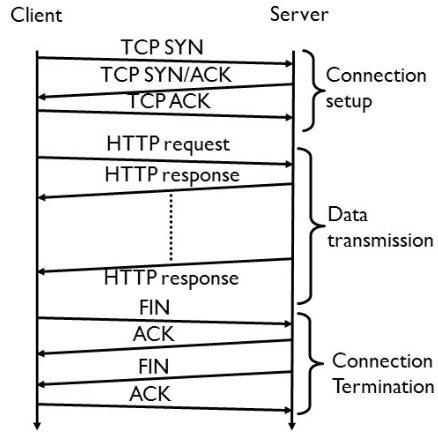
\includegraphics[width=8cm]{./02_Capitulos/02_Cap3/figures/http-flow}
\caption{Fluxo de conexão do HTTP}
\label{fig:3.2.0/http-flow}
\end{figure}

Já o MQTT é um protocolo de cabeçalhos menores, conexão persistente e menos passos para o envio de mensagem, como visto na \ref{fig:3.2.0/mqtt-flow}, por ser um protocolo feito com o objetivo de reduzir a latência, levando vantagem para a transmissão contínua de dados, em relação ao HTTP.

\begin{figure}[h]
\centering
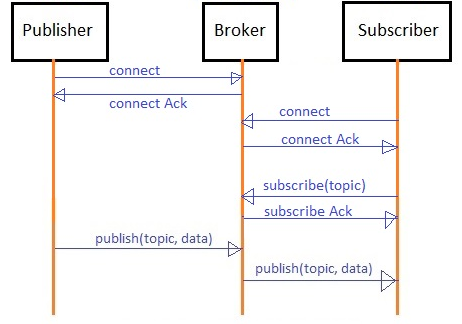
\includegraphics[width=8cm]{./02_Capitulos/02_Cap3/figures/mqtt-flow}
\caption{Fluxo da conexão do MQTT}
\label{fig:3.2.0/mqtt-flow}
\end{figure}

Abaixo na \ref{tabela:mqttxhttp} encontra-se o resumo comparativo entre os protocolos MQTT e HTTP:

\begin{table}[h!]
\caption{Comparativo MQTT X HTTP}
\resizebox{\textwidth}{!}{%
\begin{tabular}{|l|l|l|}
\hline
\textbf{Característica-Protocolo}     & \textbf{MQTT}                           & \textbf{HTTP}         \\ \hline
\textbf{Arquitetura}                  & Publish/Subscribe                       & Request/Response      \\ \hline
\textbf{Complexidade}                 & simples                                 & complexa              \\ \hline
\textbf{Segurança}                    & TSL/SSL                                 & TSL/SSL               \\ \hline
\textbf{Camada de Transporte}         & TCP                                     & TCP ou UDP            \\ \hline
\textbf{Tamanho/Formato de Mensagens} & curtas, binário com cabeçalho de 2Bytes & Grande, Formato ASCII \\ \hline
\textbf{Porta Padrão}                 & 1883                                    & 80 ou 8080            \\ \hline
\textbf{Distribuição de dados}        & 1 um para 0/1/N                         & um para um            \\ \hline
\end{tabular}%
}
\label{tabela:mqttxhttp}
\end{table}



\subsection{MQTT}
\label{subsection:mqtt}

O protocolo MQTT \cite{mqtt} foi utilizado escolhido por ser leve e ideal para aplicações em tempo real com vários dispositivos simultaneamente. É um protocolo no padrão Publish/Subscribe  ideal para definir a função de cada dispositivo seja enviando dados (Publish) ou recebendo estes (Subscribe).

Para gerenciar os clients (responsáveis pela implementação da comunicação MQTT) em cada dispositivo é necessário um servidor chamado Broker. Este foi implementado com o Mosquitto \cite{mosquitto}, um broker open source e leve capaz de ser instalado localmente e no servidor do laboratório para testes remotos.

\subsubsection{Broker}
\label{subsubsection:broker}

O Broker é o servidor do padrão Publish/Subscribe, ele efetivamente executa as ordens de publicação (publish) feita por algum cliente para os tópicos que outros clientes estão inscritos (subscribed), possui todas as listas de tópicos, é orientado a conexão e não persiste informações dos clientes, ou seja, em caso de queda de conexão, estes devem se inscrever novamente nos tópicos.

\textit{Nota: A arquitetura Broker não é exclusividade do MQTT, outros protocolos utilizam esse tipo de implementação em servidores.}


\begin{figure}[h]
\centering
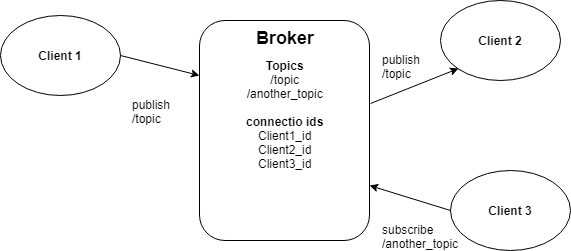
\includegraphics[width=12cm]{./02_Capitulos/02_Cap3/figures/broker_pub_sub}
\caption{Exemplo de gerênciamento de um broker}
\label{fig:3.2.0/broker_pub_sub}
\end{figure}

Na figura \ref{fig:3.2.0/broker_pub_sub}, o Broker armazena os tópicos e os ids de conexão dos clientes, 2 estava inscrito para ouvir as mensagens do tópico \textit{topic}, enquanto 3 enviava uma ordem de inscrição em \textit{another\_topic}, 1 envia ordem de publicação para \textit{topic}.


\subsubsection{Tipos de MQTT}
\label{subsubsection:tipos_mqtt}

%% Tipos de MQTT 
Com a evolução e o uso do protocolo, foram necessárias atualizações que contemplam funcionalidades que atendem  requisitos essenciais para aplicações da indústria. Como atender dispositivos que não usam a pilha TCP/IP e medidas de segurança (que serão melhor debatidas á frente). 

Existe uma gama de dispositivos que utilizam protocolos específicos, geralmente leves, para redes locais e leves para o transporte de dado, a exemplo do ZigBee \cite{zigbee}. Para isso foi criada uma versão do MQTT para atender estes tipos de protocolos, substituindo a base TCP/IP por outros protocolos destas camadas, mantendo a camada de aplicação e o padrão Publish/Subscribe.

Para resolver questões de segurança, foi criada uma variação do MQTT que adiciona camadas deste quesito ao protocolo de aplicação. Assim como o HTTPS o protocolo MQTTS é construído em cima do protocolo SSL/TLS (explicado em \ref{subsection:seguranca}), camada de segurança que também usa como base TCP/IP. Esta camada envolve o processo de encriptação dos cabeçalhos da aplicação e autenticação por passagem de certificados.

\subsection{Data Streams}
\label{section:data_stream}

Um Data Stream é uma interface que permite adicionar configurações de como o dado será enviado pelo Publisher, permitindo que este lide com os problemas causados pelo cenário, como congestionamentos, limitando o tamanho de mensagens, conversões de dados ou problemas de processamento. As configurações podem ser enviadas pelo Subscriber, permitindo um dinamismo caso acontece mudanças de cenários em algum Publisher. A configuração pode lidar com qualquer aspecto do envio de dados, como o tamanho das mensagens enviadas, ou a taxa de envio ou no próprio formato de mensagem enviado.

\begin{figure}[h!]
\centering
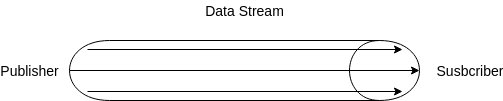
\includegraphics[width=13cm]{./02_Capitulos/02_Cap3/figures/data_stream}
\caption{O conceito de Data Stream para a abstração do transporte de dados}
\label{fig:3.1.0/data_stream}
\end{figure}

Para criar um Data Stream, basta um Subscriber estar ouvindo um tópico no formato abaixo. E um Publisher publicar neste tópico. O ID corresponde a uma identificação única que pode ser definida pelo desenvolvedor. O \textit{stream\_nome} corresponde ao tipo de Data Stream utilizado.

$$ /\{data\_stream\_id\}/stream:\{stream\_nome\} $$

Quando um Data Stream é criado, um conjunto de configurações determina como o dado será enviado, essas configurações estão contidas nos publishers dependendo da lista de Data Streams que este possui. Os Subscribers podem alterar estas configurações, baseada nas necessidades da aplicação, como problemas de processamento ou congestionamento etc.

\begin{figure}[h!]
\centering
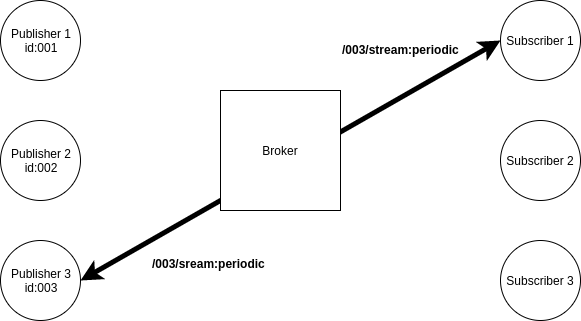
\includegraphics[width=13cm]{./02_Capitulos/02_Cap3/figures/data_stream_creation}
\caption{Um Data Stream é criado a partir do tópico \textit{/003/stream:periodic}}
\label{fig:3.1.0/data_stream_creation}
\end{figure}


Para um Subscriber enviar as alterações nas configurações basta publicar no tópico abaixo quase idêntico ao anterior. As configurações são feitas por uma string JSON \cite{json}, um conjunto de chaves-valor universalmente interpretada por várias linguagens de programação como forma de transporte de objetos de uma classe.

$$ /\{data\_stream\_id\}/configure/stream:\{stream\_nome\} $$

Existem dois tipos de Data Stream já implementados em qualquer publisher. Porém o desenvolvedor pode implementar seus próprios Data Stream dependendo da linguagem de programação utilizada:

\begin{itemize}
\item Contínuo: Data Stream padrão sem configurações definidas que publica continuamente dados;
\item Periódico: Publica dados esperando um período T antes de publicar, este período pode ser alterado;
\item Customizaveis: Criados pelo desenvolvedor, com suas próprias configurações.
\end{itemize}




\begin{figure}[h!]
\centering
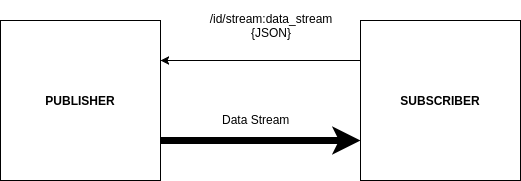
\includegraphics[width=12cm]{./02_Capitulos/02_Cap3/figures/publisher-subscriber_comm}
\caption{Comunicação entre Publishers e Subscribers por Data Stream}
\label{fig:3.2.0/pub_sub}
\end{figure}

Subscribers estão na outra ponta recebendo os dados, são capazes de enviar as configurações do Data Stream para os Publishers a chegada destes dados como um driver para a aplicação
Essas funcionalidades foram implementadas Orientadas a Objeto e são escaláveis para aplicações mais complexas que serão implementadas para o uso dos sistemas em aplicações de sensoriamento e visualização dos dados.

\subsection{Plataformas}
\label{subsection:plataformas}

%% ESP e Raspberry
Para que o sistema esteja completo, é necessário estender a interface a camada de aquisição e aplicação da pilha do IoT, para isso, foi necessário criar SDKs (Software Development Kits) para plataformas que suportem o protocolo TCP/IP. E que possam ser utilizadas em sistemas IoT. Para a camada de aplicação, foram focados em plataformas embarcadas com acesso a rede e para a aplicação, plataformas com sistemas operacionais, podendo suportar aplicações mais complexas.

A camada de aquisição apresenta implementação dos Publishers, pois são que enviam os dados, as plataformas possuem unidades de processamento e módulos de rede o que as torna ideais para publishers, porém não tão eficientes para serem Subscribers. Estes últimos são implementados na camada de aplicação, onde estão dispositivos com maiores recursos e com a função de receber dados e criar aplicações em cima desta função básica.

\subsubsection{Embarcados}
\label{subsubsection:embarcados}

Embarcados, são sistemas alimentados por baterias, sem alimentação de rede elétrica, portáveis, econômicos, com sistemas de controles geralmente feitos por microcontroladores ou microprocessadores, podendo contemplar sistemas operacionais leves. Com essa descrição, pode-se imaginar que estes dispositivos possuem processamento, energia e desempenho limitados. Para isso foi necessário a criação de uma implementação de interface leve e eficiente

Foi escolhida as plataformas microcontroladas pela arquitetura Espressif \cite{espressif}. MCUs(Micro-Controller Units) que contemplam processadores e módulos WiFi e até Bluetooth (não utilizado na interface atual), mostrados em \ref{fig:3.3.4/esp32-arch} na arquitetura do esp32, pela descrição técnica pode-se ver um poder de processamento maior que um Arduino \cite{arduino}, muito utilizado nessas aplicações e que também é compatível com a interface se adicionado shields WiFi. O ESP utiliza linguagem C++ \cite{c++} para desenvolvimento do Publisher e Data Stream, com framework Arduino que permite implementação em outras plataformas, além de uma firmware escalável, circuito open hardware e open source.

\begin{figure}[h!]
\centering
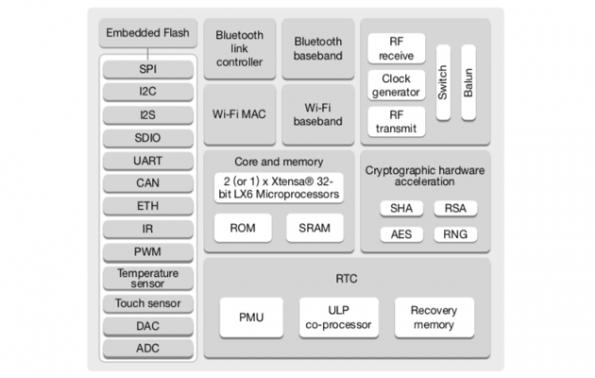
\includegraphics[width=13cm]{./02_Capitulos/02_Cap3/figures/espressif32-arch}
\caption{A arquitetura do ESP32, retirado de \cite{espressif}}
\label{fig:3.3.4/esp32-arch}
\end{figure}


Também foi implementada em Node.js (que será descrito abaixo) aplicações do Publisher para embarcados com sistemas operacionai, \cite{arm}, como Raspberry Pi \cite{raspberry-pi} e sua arquitetura mais robusta, e Intel Galileo. Permitindo multi-uso entre as funções de Publisher e Subscriber, podendo ser utilizados como Hubs ou bridges de dados. Esses consoles possuem, processadores mais potentes, periféricos, Sistemas Operacionais, assim como entradas e saídas digitais.


\subsubsection{Consoles}
\label{subsubsection:consoles}

Consoles são sistemas que contemplam sistemas operacionais, o que permitem mais liberdade para a implementação da interface. Foi escolhida então, realizar a implementação com Node.js \cite{nodejs}, um ambiente de Javascript que permite criar aplicações fora do browser, além de outras aplicações, como mobile e desktop. Possui extensas bibliotecas para HTTP e MQTT além de pipelines que permitem fácil comunicação de protocolos no mesmo processo, o que é fundamental para o conceito de escalabilidade deste projeto.


\begin{figure}[h!]
\centering
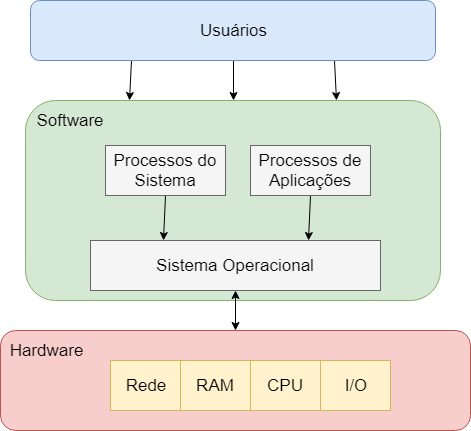
\includegraphics[width=10cm]{./02_Capitulos/02_Cap3/figures/os-diagram}
\caption{A arquitetura simplificada de dispositivos com Sistema Operacional}
\label{fig:3.3.4/os-diagram}
\end{figure}


Além disso Node.js é uma ferramenta multiplataforma, com distribuições para Windows, Linux e MAC, além de versões para embarcados de arquitetura ARM, como o próprio Raspberry Pi. Possui Módulos que permitem acessar processos do sistema operacional como ilustrado na \ref{fig:3.3.4/os-diagram} permitindo acesso a Rede além de informações do próprio sistema. O ambiente permite a implementação com programação orientada a objeto, Publishers, Data Streams, Subscribers, são instancias de classes mostradas no apêndice em \ref{section:codigos_fonte}, permitindo que a aplicação seja feita em um processo (obs: este processo pode executar outros processos, com algum overhead).  Com isso foram implementadas bibliotecas que constroem e interface sobre o MQTT, no lado Subscriber do sistema.


\section{Segurança de aplicações}
\label{section:seguranca}

%% SSL e outros tipos de encriptação de dados.
SSL \cite{ssl} (Secure Sockets Layer) é a tecnologia de segurança padrão para estabelecer um link criptografado entre um servidor da Web e um cliente. Um certificado SSL em seu servidor e um navegador se conecta a ele, a presença do certificado SSL aciona o protocolo SSL (ou TLS), que criptografa as informações enviadas entre o servidor e cliente.

O SSL opera diretamente no topo do protocolo de controle de transmissão (TCP), além de permitir que camadas de protocolo de aplicaçãoes sejam construídas por cima, agora com sob uma camada de segurança. Portanto, sob a camada SSL, as outras camadas de protocolo podem funcionar normalmente, como o HTTP e o MQTT.

Com um certificado SSL, todos os invasores poderão saber qual IP e porta e quantos dados estão sendo enviados. Eles podem terminar a conexão, mas tanto o servidor quanto o usuário poderão dizer que isso foi feito por terceiros. No entanto, eles não serão capazes de interceptar qualquer informação, o que a torna essencialmente um passo ineficaz. O invasor pode descobrir qual nome de host,mas como a conexão é criptografada, as informações importantes permanecem seguras.

Para poder criar uma conexão é requisitado um Certificado SSL. Quando você optar por ativar o SSL em seu servidor da Web, será solicitado que você responda a várias perguntas sobre a identidade do seu site e da sua empresa. Seu servidor da Web cria duas chaves criptográficas - uma chave privada e uma chave pública.

A chave pública não precisa ser secreta e é colocada em uma solicitação de assinatura de certificado (CSR) - um arquivo de dados que também contém seus detalhes, então deve-se enviar o CSR. Durante o processo de solicitação do Certificado SSL, a Autoridade de Certificação validará seus detalhes e emitirá um Certificado SSL contendo seus detalhes e permitindo que você use SSL.

Além do SSL existem outras formas de segurança. A maioria envolve encriptação. Como o uso de algoritmos de hash para encriptar as mensagens enviadas, ficando a cargo da aplicação desencriptar.

A Interface aqui construída é transparente ao SSL, ou seja, pode ser implementada em cima ou não deste protocolo, os exemplos são feitos sem esta camada, porém basta criar ou adquirir um certificado em uma autoridade de certificação e gerar as chaves. As APIs usadas contemplam da opção de usarem clients SSL.


\section{Persistência de dados}
\label{section:persistencia}

%% Bancos de dados
Os dados adquiridos pela plataforma e suas camadas, são armazenados em memórias e enviados. Memórias voláteis que podem facilmente perder dados com quedas de energia o reaproveitamento do sobre-inscrição do próprio gerenciamento do sistemas, para garantir que os dados não sejam perdidos, é necessário que o sistema possua persistência, uma forma de memória não-volátil que armazene os dados sem energia.

Essa persistência é implementada com Banco de Dados, estruturas que organizam o armazenamento de dados persistentes em arquivos. Um Banco de dados é uma basicamente uma aplicação, um serviço do sistema que recebe requisições de rede e escreve ou lê dados em um arquivo. Existem inúmeras formas de implementação e protocolos de comunicação para Bancos de Dados. Porém todos eles seguem abstrações em comum.

Um banco é composto por duas ferramentas. O Motor e o Arquivo de dados. O motor é quem realiza as ações sobre o arquivo, é o sistema de gerenciamento. Recebe as requisições e aplica algoritmos de escrita de dados eficientes no arquivo para armazenar os dados em uma estrutura definida. Um Banco de dados pode possuir vários motores, cada um com algum algoritmo que varia a eficiência e o tempo de escrita e/ou leitura dependendo do dado recebido.

\begin{figure}[h!]
\centering
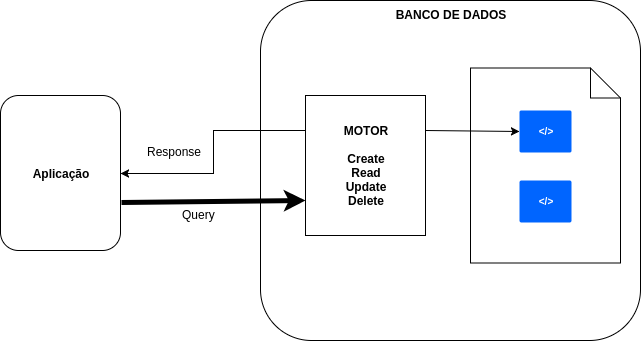
\includegraphics[width=12cm]{./02_Capitulos/02_Cap3/figures/Database_Arch}
\caption{A arquitetura de um banco de dados}
\label{fig:3.3.5/database_arch}
\end{figure}

O Arquivo é o documento onde os dados são armazenados, na estrutura definida. Possuem formatações de dados específicas de cada tipo de banco, seguindo uma abstração. O formato do armazenamento de dados, define e limita eficiência do motor, então e necessário a escolha adequada de algoritmo para uma maior eficiência da leitura do arquivo. Como em \ref{fig:3.3.5/database_arch} a aplicação envia uma solicitação de criação ou leitura ou atualização ou remoção (CRUD - Create, Read, Update, Delete) e o motor lida com os dados, armazenando-os em uma determinada estrutura no Arquivo.


 
\section{Bancos para Aplicações IoT}
\label{section:bancos_IoT}

Na área de Bancos de Dados (ou DBs), com escopo focado em IoT, há um porém. Para a estruturação de uma aplicação eficiente, não se deve usar qualquer tipo de banco. Devem-se escolher motores e estruturas de bancos adequadas para a aplicação. Não exite um critério definitivo que guia o desenvolvedor para melhor escolha. Mas algumas características de bancos de dados podem ser exploradas em aplicações IoT, formando um DB eficiente para tal.

Como pode ser observado em \cite{Damodaran}, uma aplicação eficiente de Bancos e IoT está ligada ao tempo de inserção de dados no banco,  o tempo total em que a aplicação leva para enviar, aplicar a busca de onde o dado deve ser inserido no documento e de fato armazenar, podem ser feitas várias inserções de pequenos pacotes de dados, dependendo do tamanho da mensagem. Esta característica está ligada ao motor do banco, que determina como o dado será armazenado, e quanto ele leva para escrever o dado no documento. A maioria dos dados são armazenados em estruturas B+Trees \cite{b-tree}, porém pode-se observar em \cite{Damodaran} que a estrutura LSM Tree \cite{O'Neal-Gawlick-Cheng} possui maior eficiência na escrita.


\begin{figure}[h!]
\centering
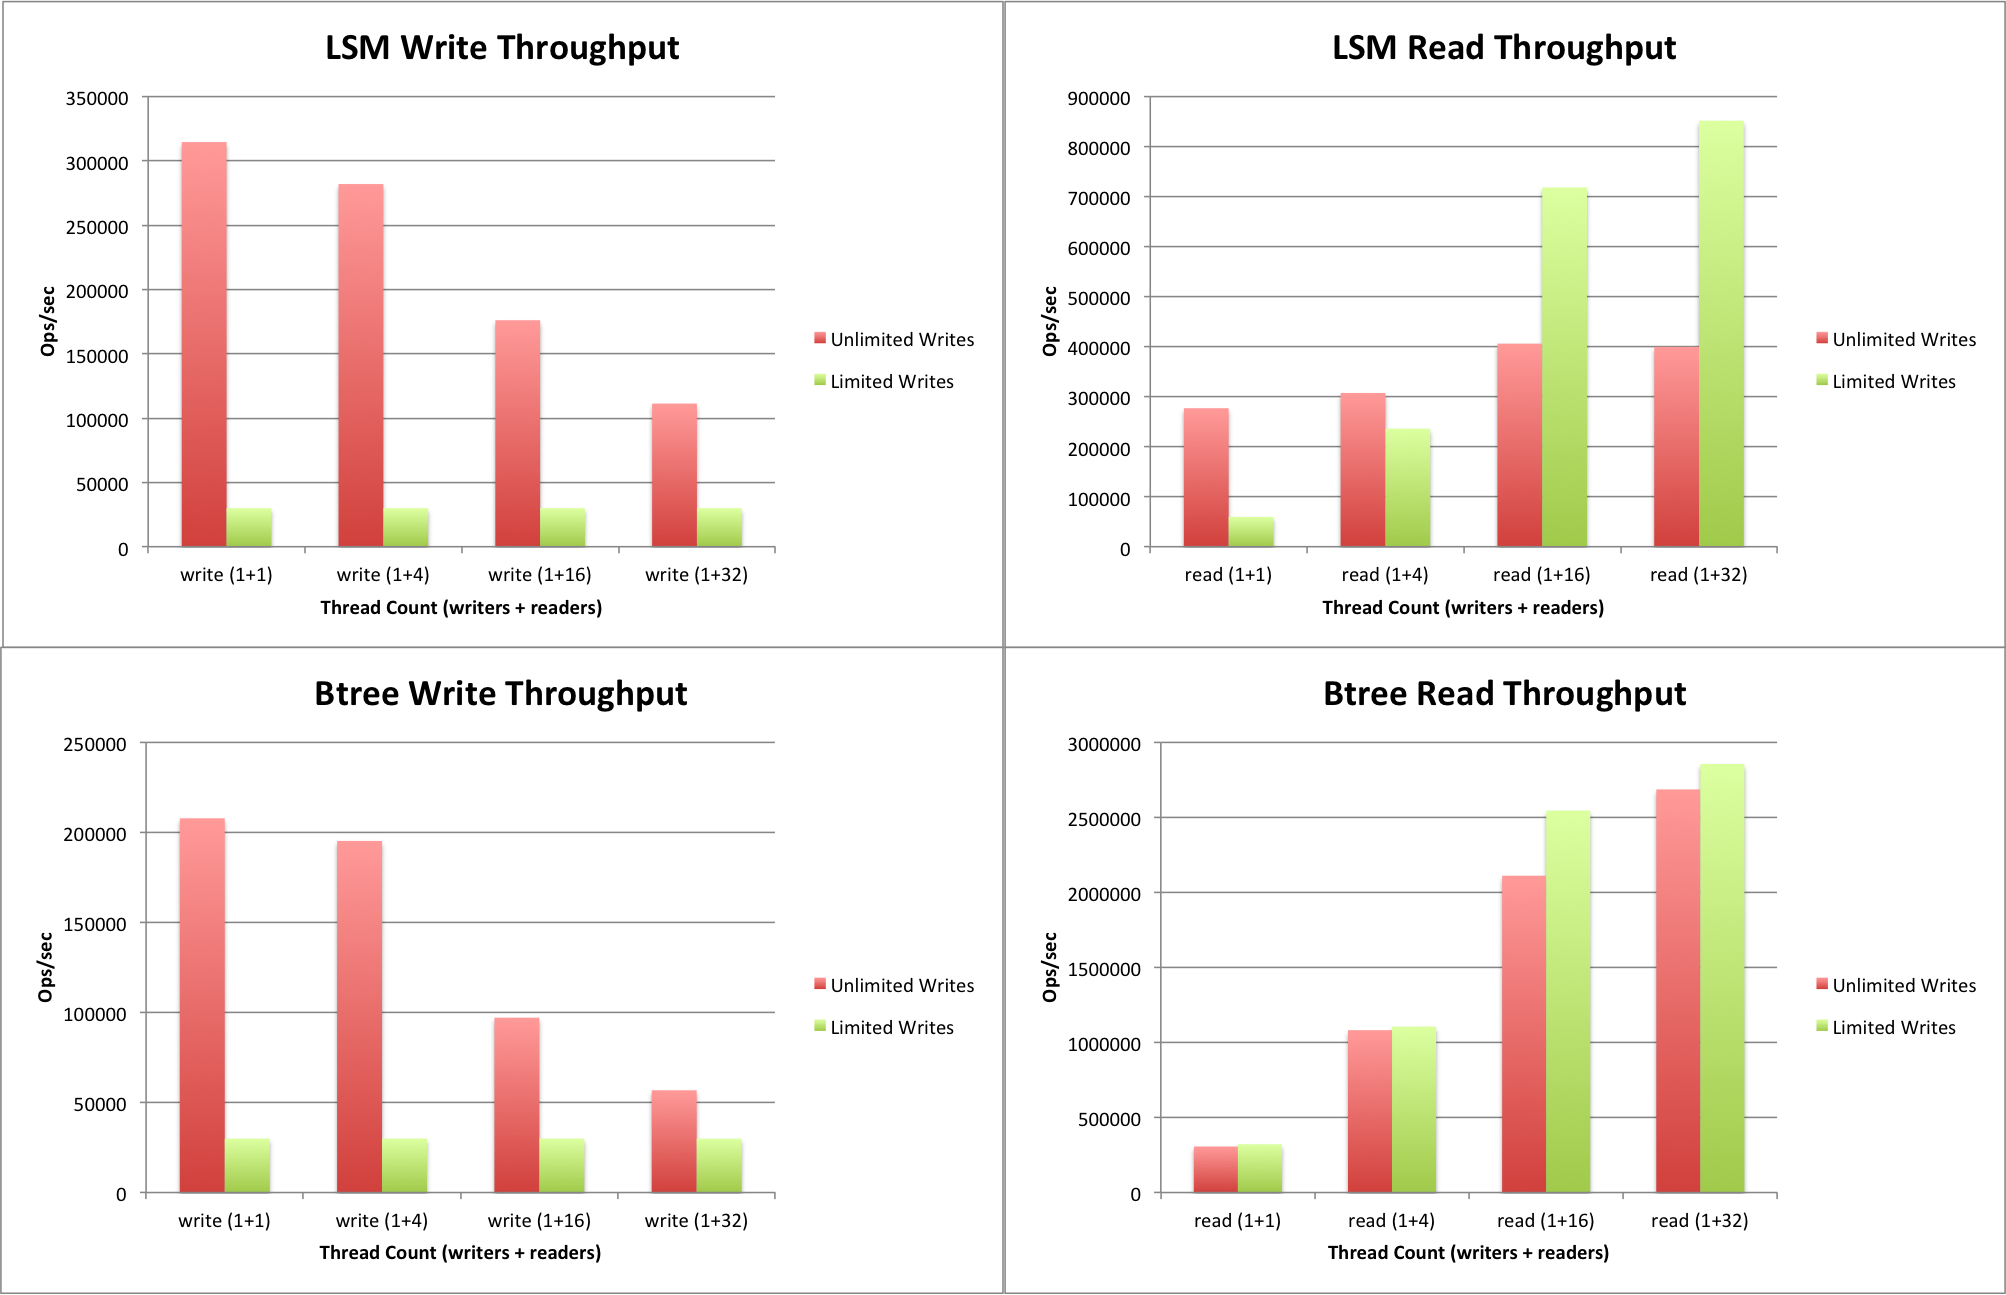
\includegraphics[width=13cm]{./02_Capitulos/02_Cap3/figures/LSM_btree}
\caption{Comparação de Escrita e Leitura entre LSM e B+, retirado de \cite{btrees-vs-lsmtrees}}
\label{fig:3.3.5/b-lsm}
\end{figure}

Comparando as duas estruturas, como mostrado em \ref{fig:3.3.5/b-lsm}, percebe-se que a estrutura LSM sustenta até 2x mais inserções da estrutura B+, hoje os Bancos de Dados modernos utilizam desta vantagem, devida a nova tendência de aplicações de coletar dados constantemente, o que leva a operação de escrita no banco ter mais importância e ocorrências que a leitura e explica a migração para a estrutura LSM.

Existem várias abstrações de Bancos de dados. Em \cite{Rautmare-Bhalerao} compara-se e conclui-se que o banco MongoDB, um banco NoSQL possui um tempo de resposta de inserção menor que o MySQL (bancos relacionais), porém o último é mais estável. De fato bancos NoSQL são, em geral, mais leves, possui uma flexibilidade maior para lidar e estruturar dados, o que fazem estes tipos de Banco mais favoráveis a aplicações de IoT. Porém outras estruturas como um banco divido em timescale mostram-se eficientes SQL ou não.

Outros aspectos podem contribuir para a eficiência de persistência de dados. Criar bancos locais diminuem a latência e a necessecidade de conexão, aumentando a capacidade de inserção de dados, além de ser uma forma de backup de dados. Um banco local, geralmente fica em uma plataforma como em \cite{Paethong-Sato-Namiki}, são bancos leves em aplicações de baixo consumo, devido a capacidade de processamento limitada. Seu papel é geralmente para armazenar os dados quando não há conexão, e quando esta é restabelecida os dados são enviados para um banco remoto com mais capacidade de processamento e aplicações. %% Falar sobre bancos locais.

Dentre os bancos estudados, alguns se destacam como o Cassandra, usado pela Netflix para coletar dados sobre o comportamento do usuário na plataforma ou o InfluxDB, um banco de arquitetura TimeScale, feito para aplicações em tempo real. Mas para esse projeto, foi utilizado o MongoDB \cite{mongodb}, um banco NoSQL, leve, de facil integração com as plataformas utilizadas e que posui implementações de motores que priorizam a eficiência na escrita de dados, como a LSM tree.

\section{Indexação de dados e Timestamp}
\label{section:timestamp}

Na seção anterior foram discutidos estruturas da organização de dados e o formato de armazenamento de dados como o formato de Documento e TimeScale. É importante que estes formatos tenham formas eficientes de indexação, de modo a facilitar a busca e a análise de dados.

Em uma aplicação de IoT, que envolve coleta de dados em tempo real, é fundamental, independentemente do formato escolhido, a informação de quando este dado foi colhido (data e hora). Isto permite a análise dos dados ao longo do , conforme forem armazenados. Aplicações de decisão e análise utilizam ferramentas estatística com base nas ocorrências temporais, projetando previsões e classificação. No projeto atual, foi implementado o MongoDB um banco de dados de documentos. Cada documento é indexado por uma identificação única como mostrado na \ref{fig:document-model}, permitindo também criar relações entre documentos.

\begin{figure}[h!]
\centering
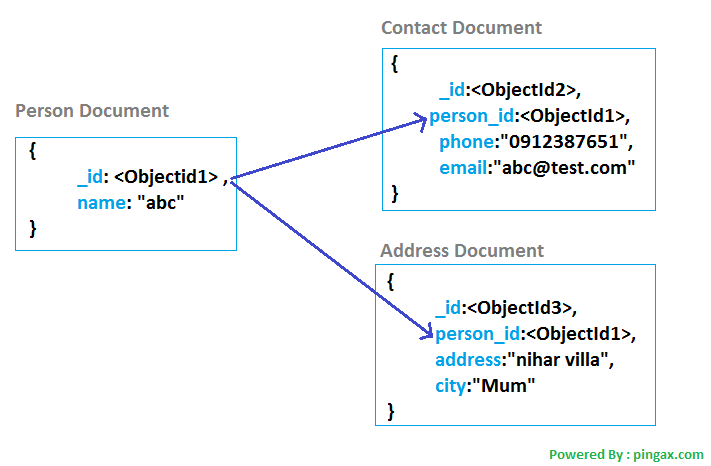
\includegraphics[width=10cm]{./02_Capitulos/02_Cap3/figures/document-model}
\caption{O formato de documento no MongoDB}
\label{fig:document-model}
\end{figure}

O banco também permite adicionar outros parâmetros de indexação definidos pelo desenvolvedor, foi utilizado desta funcionalidade para adicionar um campo de Timestamp, uma informação de data e hora da inserção no banco. Na implementação foi utilizado o formato Unix Timestamp, o número de milisegundos que se passaram desde 1 de Janeiro de 1970 ás 00:00:00 (UTC), a \ref{fig:document-timestamp} ilustra o formato de documento completo usado no sistema, o campo de dados é definido pelo desenvolvedor. 

\begin{figure}[h!]
\centering
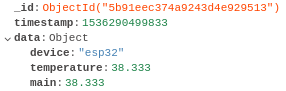
\includegraphics[width=8cm]{./02_Capitulos/02_Cap3/figures/document-timestamp}
\caption{Adição de parâmetro de timestamp em milisegundos ao documento}
\label{fig:document-timestamp}
\end{figure}

Vale ressaltar a existência de uma nova geração de Bancos de Dados TimeScale, um formato parecido com o de Documento, porém com indexação feita por Timestamp ao invés de uma chave única. Em destaque o Banco InfluxDB, que possui estrutura LSM-Tree além de ser um banco TimeScale, o que o faz ser utilizado cada vez mais em aplicações IoT.